\section{Cold dwarf remnants and tidal inheritance}
\label{sec:crater}

Crater II combines a large projected half-light radius with a small stellar
velocity dispersion. The moving-Milky-Way-plus-LMC calculation produces a
surviving stock remnant with
\begin{equation}
\sigma_{\rm los}=2.36\,\kms,\quad R_h=0.86\,\mathrm{kpc},\quad
M_*=3.2\times10^5\Msun,\quad f_{\rm tail}=0.23.
\label{eq:craterbest}
\end{equation}
A second well-ranked state gives
$(2.18\,\kms,1.24\,\mathrm{kpc},4.4\times10^5\Msun,0.38)$.
The comparison data used by the likelihood are
$(2.7\pm0.3\,\kms,1.066\pm0.084\,\mathrm{kpc},
3.2\pm1.0\times10^5\Msun,0.23\pm0.08)$.
The first state matches the dispersion, mass, and adopted tail statistic
well, while its radius is about 19\% low. The second is larger and has
more stellar debris. \source{G3, G4}

Against the specified NFW halo ensemble, the moving-LMC comparison gives
$B=1.98\times10^8$ for 0.3-dex halo-mass scatter and
$B=2.62\times10^5$ for 0.5-dex scatter when the fractional model error is
10\%. These values have been recomputed from the saved run outputs for
this document. They quantify a preference for the stock construction
within this numerical experiment.

\subsection{Which satellites keep their stock}

A satellite has its own cells only where its own baryonic field exceeds
the host's. At the three-dimensional half-light radius the ratio of the
Milky-Way law field to the dwarf's own law field is $5.5$ for Sextans,
$2.5$ for Draco, $2.0$ for Ursa Minor and $1.7$ for Carina, which keep
their pre-infall stock, and $0.98$ for Sculptor, $0.38$ for Fornax,
$0.20$ for Leo~II and $0.09$ for Leo~I, which relax. Scored on the
GravSphere central densities $\rho(150\,{\rm pc})$ \cite{read19}, this
assignment gives $\chi^2=10.4$ over the eight dwarfs, against $17.2$
for retained stock throughout and $44$ for relaxed stock throughout.
Ten of the $256$ retained or relaxed assignments reach
$\chi^2\le10.4$; the best, $5.7$, also retains Leo~II. The
classification holds for Milky-Way baryonic masses of
$5$--$6\times10^{10}M_\odot$, cap ratios of $10$--$20$, projected or
three-dimensional radii, and Newtonian or law fields, with Sculptor on
the boundary. \source{G12}

A dwarf whose main progenitor never crossed the release gate of
Section~\ref{sec:cosmology} keeps its committed allocation, and its stock
stays collisionless. Over 22 Local Group dwarfs with half-light masses
from the Local Volume Database, relaxed masses from contact runs, and gate
crossing from the mean accretion history of Fakhouri et al. (2010), this
combined assignment gives $\chi^2=21.7$ at the reference gate of
$17\,\kms$ and $25.4$ at $14\,\kms$. \LCDM\ halos with supernova heating
at the published coreNFW calibration give $24.0$, and NFW halos without
heating give $30.0$. Over plausible accretion histories, M31 baryonic
masses and the two published Tucana dispersions, the combined assignment
spans $18.5$--$29.2$ and heating spans $23$--$25.5$; these data do not fix
the gate. \source{G12}

\subsection{Why size and dispersion must be explained together}

In a dispersion-supported system, random stellar velocities provide
support against gravity. Under equilibrium and approximate spherical
symmetry, a useful scale estimate is
\begin{equation}
M(<r_{1/2})\simeq\frac{3r_{1/2}\sigma_{\rm los}^2}{G}
\simeq\frac{4R_h\sigma_{\rm los}^2}{G},
\label{eq:wolf}
\end{equation}
where $r_{1/2}\simeq4R_h/3$ is the three-dimensional half-light radius.
For the adopted Crater II values this gives roughly
$7.2\times10^6\Msun$. The estimate is a guide to the required depth of
the central potential; a tidally disturbed galaxy requires direct
modeling. \cite{wolf}

Reducing a halo's central mass can cool the stars, but its tidal response
can also contract or destroy the stellar distribution. A successful model
must retain a diffuse body while reducing its binding potential, and
must leave the right amount of visible debris. A dispersion fit at an
incorrect radius addresses only part of the problem.

\subsection{Initial conditions and the physical stock profile}

The stellar progenitor is a Plummer sphere,
\begin{align}
\rho_*(r)&=\frac{3M_*}{4\pi b^3}
\left(1+\frac{r^2}{b^2}\right)^{-5/2},\\
M_*(<r)&=M_*\frac{r^3}{(r^2+b^2)^{3/2}}.
\end{align}
Its projected half-light radius is $b$. The progenitor's isolated stock is
initialized from
\begin{equation}
M_R(<r)=\min\left\{M_*(<r)
\left[\nu\!\left(\frac{GM_*(<r)}{a_0r^2}\right)-1\right],
C_RM_*\right\},
\label{eq:dwarfstock}
\end{equation}
with $\nu(y)=(1-e^{-\sqrt y})^{-1}$ and $C_R=3000$.
The differentiated density is tapered by $e^{-(r/12\,\mathrm{kpc})^2}$.
The cap and taper are specified modeling inputs tied to the proposed
history and its numerical realization. They are not independently
measured halo properties of Crater II.

The central form explains why stock responds differently from a cusp.
For $r\ll b$, the Plummer mass scales as $r^3$, so $g_b\propto r$.
In the low-acceleration limit, $\nu-1\propto r^{-1/2}$. Consequently
\begin{equation}
M_R(<r)\propto r^{5/2},\qquad \rho_R(r)\propto r^{-1/2}.
\end{equation}
This is shallower than the $r^{-1}$ inner density of an NFW halo. The
outer stock is extended and weakly bound. Tides can remove substantial
stock and lower the stellar velocity scale without forcing the same
stellar contraction as in the tested NFW models.

Both stars and stock are initialized through isotropic Eddington
distribution functions in the combined potential. This matters because
the initial density profile alone does not specify stellar velocities.
For relative potential $\Psi=-\Phi+\Phi(\infty)$ and relative energy
$\mathcal E=\Psi-v^2/2$, the inversion can be written
\begin{equation}
f(\mathcal E)=\frac{1}{\sqrt8\,\pi^2}\frac{d}{d\mathcal E}
\int_0^{\mathcal E}\frac{d\rho/d\Psi}{\sqrt{\mathcal E-\Psi}}\,d\Psi.
\end{equation}
At a sampled radius, speeds are drawn with probability proportional to
$v^2f(\Psi-v^2/2)$. The code evaluates the inversion on a finite radial
grid and clips negative numerical values of $f$ to zero; equilibrium and
resolution controls are needed to assess this approximation.
Equilibrium phase-space sampling avoids using an arbitrary initial
velocity dispersion as a hidden fit parameter. \source{G1, G3}

\subsection{The orbit and the LMC perturbation}

The calculation uses the present position, distance, radial velocity, and
proper motion to infer a past orbit in each gravitational model. The
adopted Crater II inputs are $D=117.5\,\mathrm{kpc}$,
$v_{\rm los}=87.5\,\kms$, and
$(\mu_{\alpha*},\mu_\delta)=(-0.07,-0.11)\,\mathrm{mas\,yr^{-1}}$.
The stock Milky Way contains $6\times10^{10}\Msun$ of baryons and a
retained profile with $C_R=14$.

The moving LMC carries $3\times10^9\Msun$ of Plummer baryons and its
retained profile, capped at $1.02\times10^{11}\Msun$ in total.
The trajectory includes a specified Chandrasekhar friction term and
the acceleration of the Milky Way. In this calculation Crater II's latest
pericentre is 25.3 kpc, 1.68 Gyr before the present, in the stock host;
the NFW comparison gives 24.9 kpc. The models use the same observed
phase-space inputs, but their host potentials give distinct orbits.
\source{G4}

Only first-pericentre stock progenitors survive in the sampled moving-LMC
grid. Its best state begins with twice today's stellar mass and
$0.7R_{h,\rm obs}$. The next state begins with four times today's mass
and $R_{h,\rm obs}$. The agreement includes inference over progenitor
mass, size, and infall age within a prior-weighted grid.

A rough tidal-radius estimate makes the mechanism clear. For a small
satellite on a circular orbit of radius $R$ in a spherical host,
\begin{equation}
r_t\simeq R\left[
\frac{m(<r_t)}{[3-d\ln M_H/d\ln R]M_H(<R)}
\right]^{1/3}.
\end{equation}
The real orbit is eccentric and the LMC makes the potential time
dependent, so the simulation integrates the forces directly. Near
pericentre, the strongest differential field removes the weakly bound
outer stock. The retained stellar body then responds to a shallower
potential. Its final dispersion is an output of this evolution.

\subsection{What the numerical experiment actually resolves}

The shared solver follows 40,000 stock or dark particles and 10,000 stellar
particles with a one-Myr leapfrog step and 0.03 kpc softening. Self-gravity
is computed through a monopole about the density centre. The external
Milky Way and LMC fields are applied to the particles. This is a
collisionless particle experiment with spherical internal force
resolution, not a full unrestricted tree-gravity calculation.

The comparison uses NFW subhalos with a Moster stellar-to-halo mass prior
and the Dutton--Macci\`o median concentration relation. Progenitor masses
are one, two, or four times today's stellar mass; sizes are $0.7$, $1.0$,
or $1.5$ times the observed half-light radius, weighted by the stated
size--mass prior. The infall-age grid counts pericentric passages.
The enlarged halo grid includes masses far below the central
abundance-matching expectation. \source{G3, G4}\cite{moster,dutton}

The NFW models approach the observed dispersion at inferred infall masses
around $10^{7.4}$--$10^{7.7}\Msun$, about two dex below the reference
abundance-matching relation. Their radii then lie near 0.76--0.78 kpc and
their dispersions near 3.2--3.5 $\kms$. The two-dex statement describes
the required prior displacement in this model family. It is not a universal
proof that a galaxy could never have formed in such an object: gas
retention, early cooling, concentration, and assembly history also matter.

\subsection{Tail counts and the measurement procedure}

The MAGIC photometric sample contains 162 candidate red-giant members,
37 of them in the tails, giving $37/162=0.2284$. The reported stream width
is about $0.8^\circ$, and the tails extend beyond the observed footprint.
These are population- and selection-dependent measurements. A candidate
count is not automatically a complete fraction of all stellar mass.
\cite{atzberger}

The grid likelihood uses $f_{\rm tail}=0.23\pm0.08$ and a statistic counting
stars beyond $3R_{h,\rm obs}$ within a three-dimensional radius of about
14.4 kpc. The central dispersion is measured from bound stars within
$1.5R_h$ in projection. These definitions can be reproduced from the
simulation, but the observing program does not have direct access to a
bound-particle label or a spherical three-dimensional membership cut.
A final comparison needs the photometric footprint, candidate selection,
velocity errors, gradient subtraction, and foreground model applied to
mock observations.

Independent spectroscopy now confirms cold central kinematics and
provides a stream-to-body dispersion ratio. Limberg et al. report
$2.51^{+0.33}_{-0.30}\,\kms$ for the body and
$5.74^{+0.98}_{-0.83}\,\kms$ for the stream. Their own simulations find
the dispersion ratio difficult for standard-concentration cusps, while
cored or low-concentration halos can reproduce it. The stock model should
predict this ratio and the stream width as additional observables.
\cite{limberg}

\subsection{The strength and the scope of the model comparison}

For an observable $O_j$, the grid uses an effective error
$s_j^2=\sigma_{j,\rm obs}^2+(f_{\rm mod}O_{j,\rm model})^2$ for
dispersion and radius. Its Gaussian likelihood includes the $1/s_j$
normalization. With fixed observational errors for stellar mass and
tail fraction,
\begin{equation}
\mathcal L(\theta)\propto
\prod_j\frac1{s_j}
\exp\left[-\frac{(O_{j,\rm model}(\theta)-O_{j,\rm obs})^2}{2s_j^2}\right].
\end{equation}
Destroyed states receive zero likelihood. The evidence is a discrete
prior average, $Z=\sum_iw_i\mathcal L_i/\sum_iw_i$ for the normalized
grid, with the documented Gaussian mass-prior quadrature for the extended
halo tail. The Bayes factor is $B=Z_{\rm stock}/Z_{\rm NFW}$.

\begin{center}
\small
\begin{tabular}{lrr}
\toprule
Fractional model error & With LMC, 0.3-dex mass scatter & With LMC, 0.5 dex\\
\midrule
10\% & $1.98\times10^8$ & $2.62\times10^5$\\
20\% & $2.99\times10^3$ & $9.26\times10^2$\\
30\% & $1.55\times10^2$ & $9.42\times10^1$\\
\bottomrule
\end{tabular}
\end{center}

The preference remains in the same direction throughout these sensitivity
checks, while its numerical magnitude changes by several orders of
magnitude. The quoted large factors require the 10\% model-error assumption. The
numerical errors, force approximation, orbit uncertainty, and observation
mapping should determine that error budget independently.

\begin{figure}[htbp]
\centering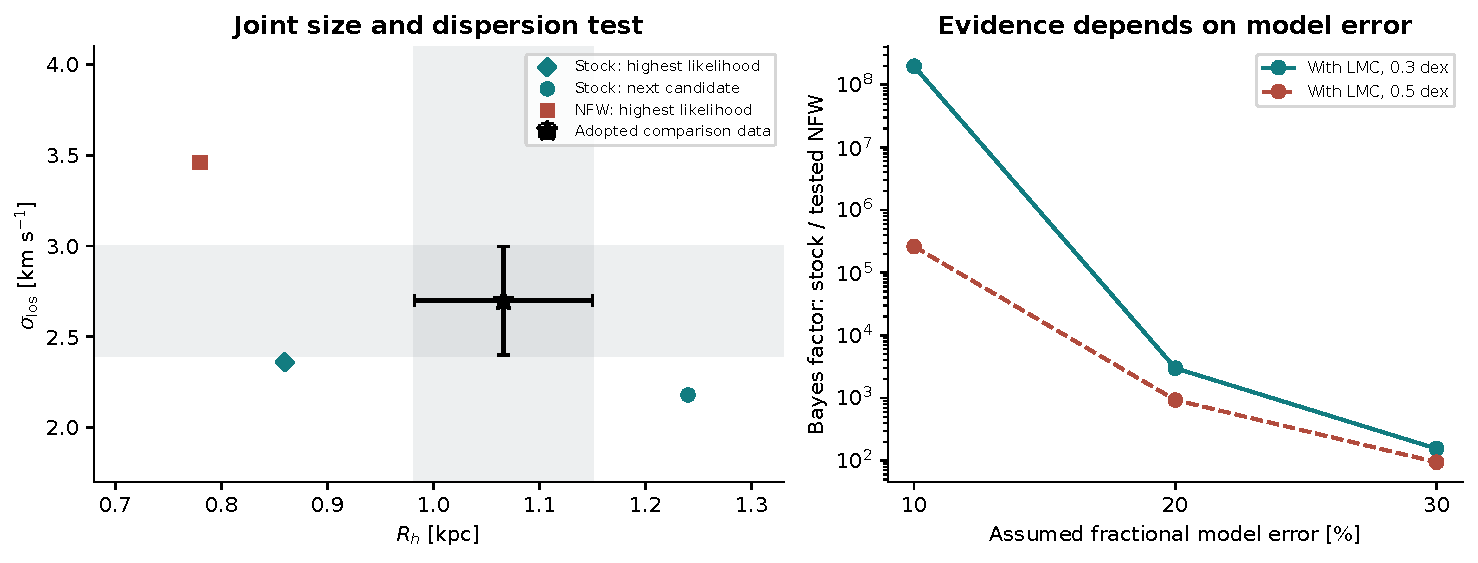
\includegraphics[width=\textwidth]{figures/crater.pdf}
\caption{The moving-LMC Crater II comparison and its dependence on the
assumed model error. The left panel emphasizes the joint size and
dispersion constraint. The evidence calculation also uses stellar mass
and the adopted tail fraction. The two halo priors use the same saved
particle trajectories.}
\end{figure}

The archived record describes a hash-locked core protocol preceding the
comparison campaign. The moving-LMC extension and enlarged mass priors
are documented follow-ups.
The present file hash matches the stored registration hash. A matching
hash verifies file identity; by itself it does not independently certify
the historical ordering of executions. \source{G3, G4, G6}

The tested alternative consists of cuspy halos at a prescribed
concentration relation. It does not cover the full range of concentration
scatter, feedback-induced cores, or every dark-matter model. Crater II
therefore favors the stock model strongly over this specified alternative.
It does not establish odds against the entire \LCDM\ framework.

The moving-LMC satellite grid was reweighted with ten, twenty, and
thirty percent model uncertainty. At thirty percent the Crater II
stock/NFW evidence falls to 94--155 from $2.6\times10^5$--$2.0\times10^8$
at ten percent; Antlia 2 rises from 0.007--0.019 to 0.69--0.74.
The grid does not implement the new conservative joint-stock contact
or span broad cored-halo alternatives. Its evidence remains conditional
on the specified histories, priors, and error budget. \source{U1, S14}

\subsection{Antlia 2: a recently disturbed system still requires a successful mock observation}

Antlia 2 has a measured dispersion
$5.98^{+0.37}_{-0.36}\,\kms$ after fitting a velocity gradient.
The gradient is $5.72^{+0.60}_{-0.56}\,\kms$ per degree. Ji et al. find
evidence of tidal disturbance and show that its orbital interpretation
requires the LMC-induced reflex of the Milky Way. \cite{ji}

In the available moving-LMC stock runs, five of the 27 states survive.
The best bound remnant has $\sigma=3.48\,\kms$,
$R_h=2.41\,\mathrm{kpc}$, and $M_*=9.4\times10^5\Msun$.
Its most recent pericentre is about 0.79 Gyr ago. The NFW comparison can
approach the adopted observables using low-mass halos; on the original
bound-star likelihood it is favored over the stock by about 50--140.
\source{G4}

The suggestion that Antlia 2 has not had enough time to reveal a settled
internal dispersion can be made quantitative. Using its observed radius
and dispersion,
\begin{equation}
t_{\rm cross}\sim\frac{R_h}{\sigma}
\simeq0.978\,\frac{2.92}{5.98}\,\mathrm{Gyr}
\simeq0.48\,\mathrm{Gyr}.
\end{equation}
The elapsed time is only about 1.6 such crossing times; using the best
stock remnant gives a crossing time near 0.68 Gyr. A dynamically disturbed
state is plausible. This concerns time since disturbance, not the age
of its stellar population.

The available approximate mock analyses show that unbound members and
velocity-mixture choices can move the inferred dispersion substantially.
They even change the relative ranking of the tested models. That is a
reason to use the observed selection and membership procedure. A
quantitative explanation of the measured 6 $\kms$ remains to be established.
The collisionless integrations already contain the tidal evolution;
a successful non-equilibrium account must show how that evolution produces
the measured dispersion, gradient, density profile, and membership sample
together. Antlia 2 remains an unresolved test of the current construction.
\source{G6}

\subsection{What the Crater II result changes}

The successful stock trajectories show that a diffuse cold remnant can
emerge from a specified positive mass component tied to baryonic history.
This challenges the assumption that the excess gravity of such a dwarf
must be recalculated from its present stars, or must be supplied by a
standard-concentration NFW subhalo with the adopted abundance prior.
The mechanism is explicit: outer stock is stripped, the central potential
weakens, and a substantial stellar body survives.

The next discriminants are the full stream structure, the velocity
distribution including unbound stars, and an independently controlled
model-error budget. They test the same history that produced the central
dispersion, so they can constrain the model without introducing a new
halo normalization for each observable.
